\section{Implementation and Evaluation}


\textbf{Phones and Placements.} We use Huawei Nexus 6P Android smartphone to collect user data. Since we mainly use the microphone data to detect the syllable nuclei time, we do not require a high sampling frequency of audio data. Indeed, we only record the data at 8000 Hz (telephone quality). For the motion data, however, the sample frequency is the higher the better. The Nexus 6P is manufactured in 2015, but we have updated its operating system to Android Orea (API level 26), which is released in 2017. By calling the \texttt{getMinDelay()} function, we found the minimum delay allowed between two motion sensor events is 2500 microsecond, which is a sample frequency of 400 Hz. Therefore, we use 400 Hz for both gyroscope and accelerometer. As shown in Fig.~\ref{fig:use}, a smartphone user places his device to his throat tightly so that conductive vibrations can be measured. The data collection app is shown in ~\ref{fig:defendappa}.

\begin{figure}[H]
	\centering
	\begin{minipage}{.3\linewidth}
		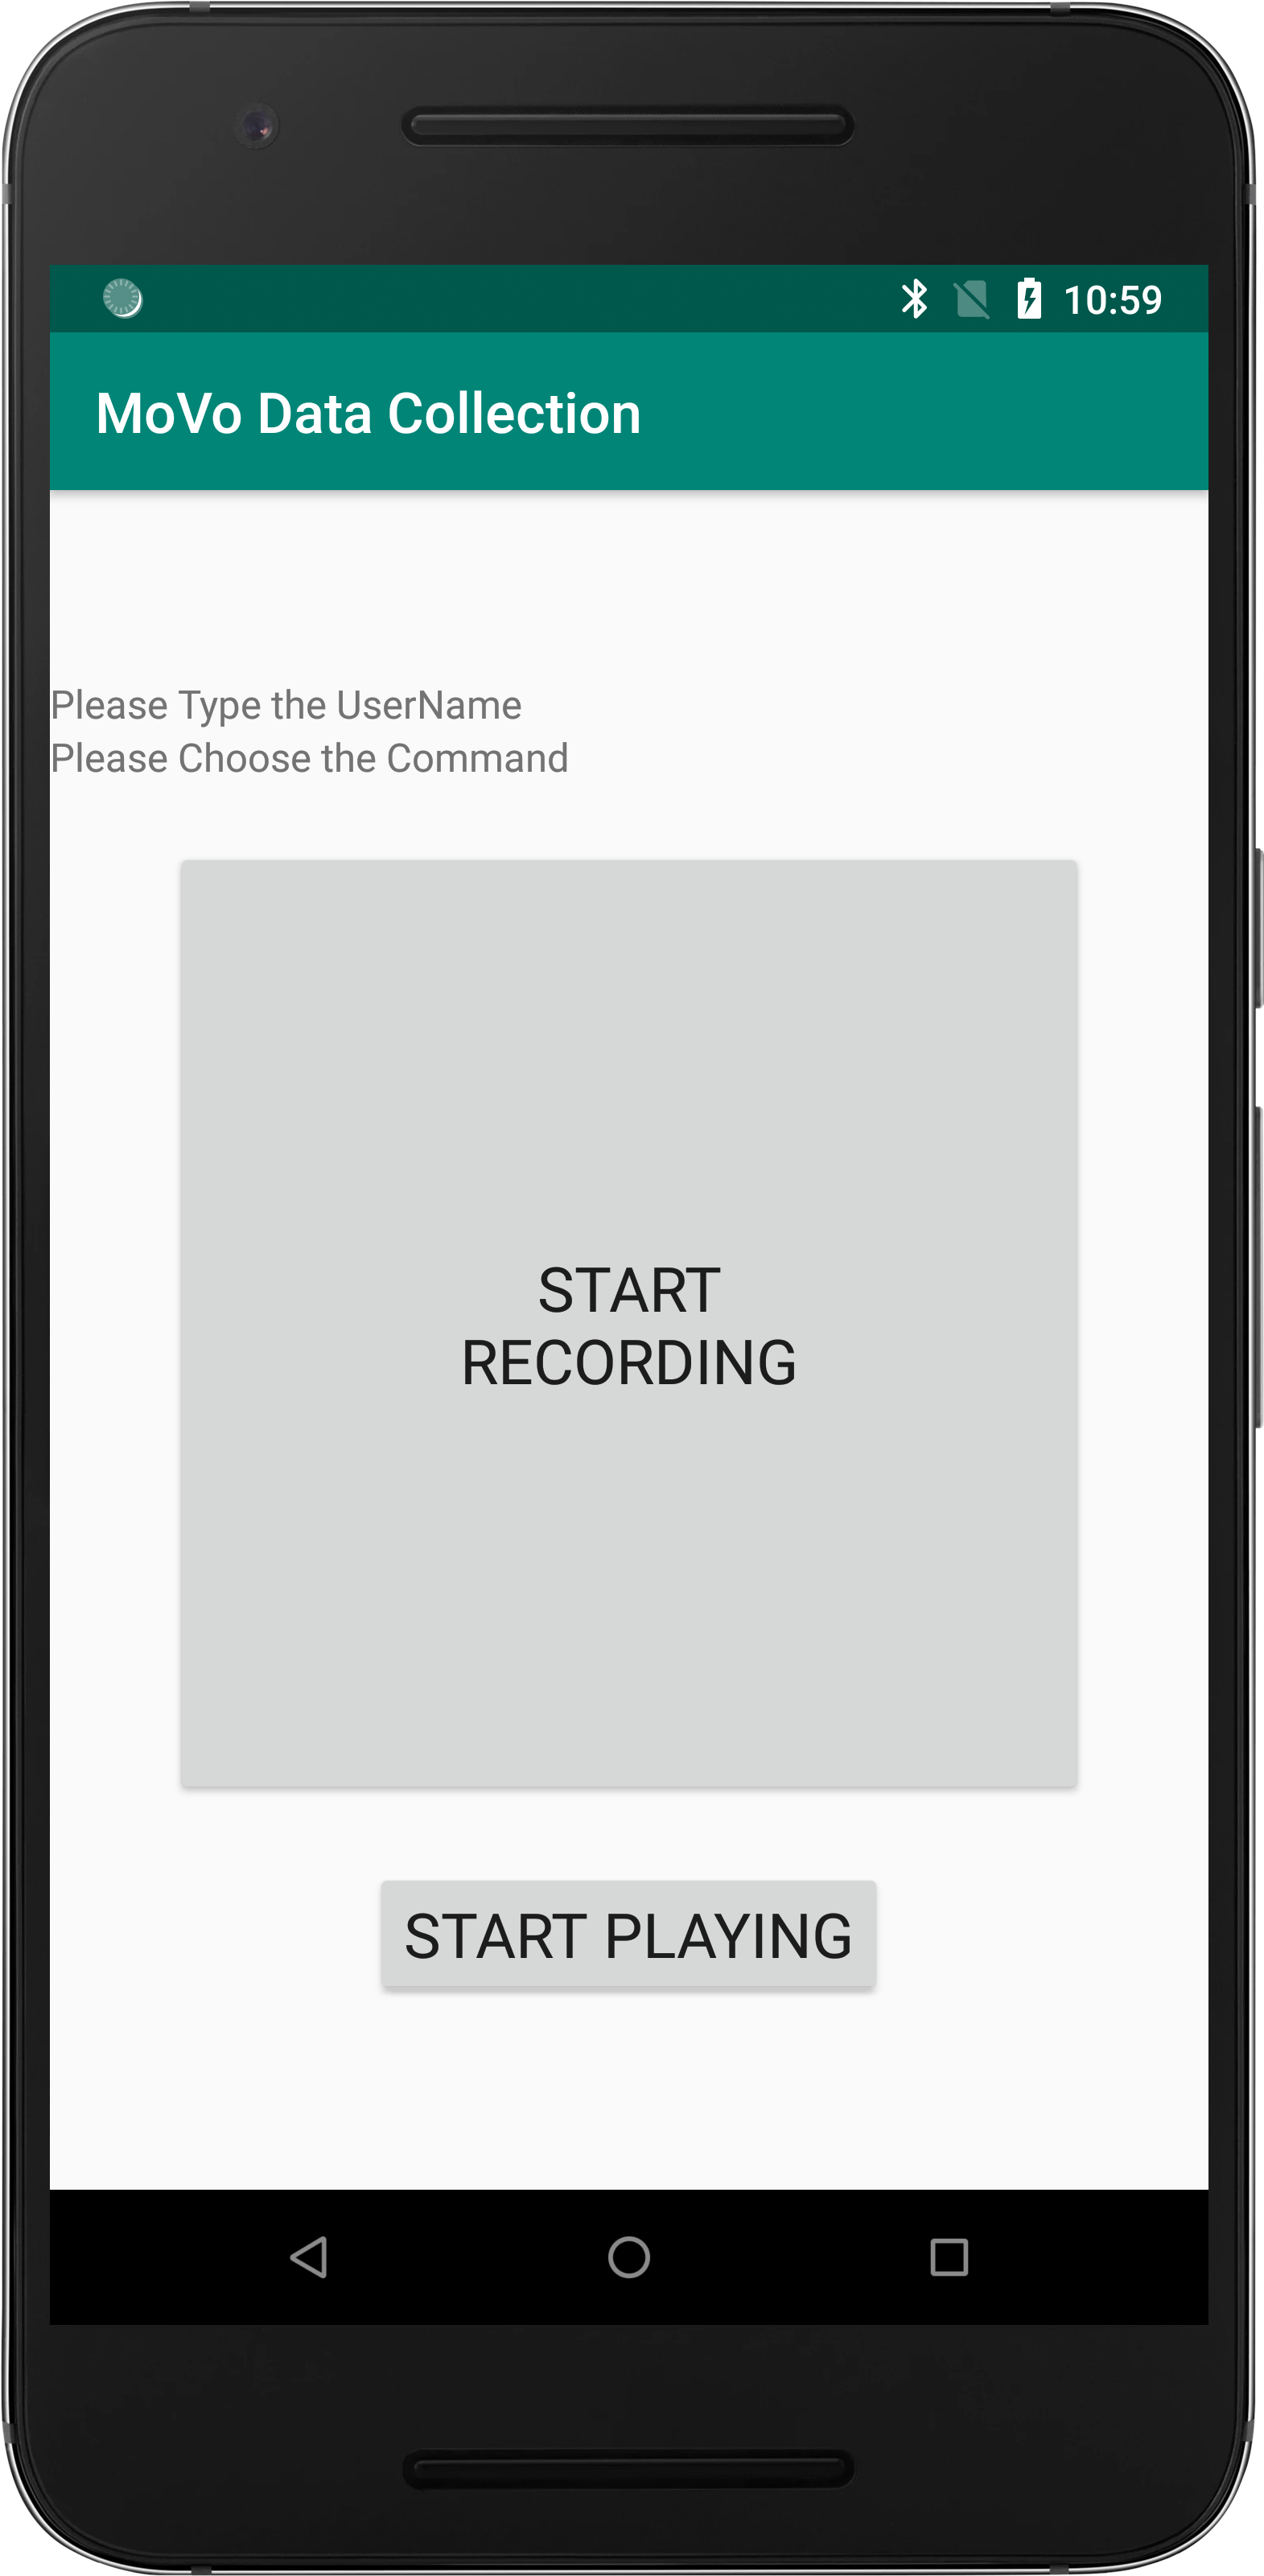
\includegraphics[height=.4\textheight]{MoVoData}
		\subcaption{{\mv} Data Collection}\label{fig:defendappa}
	\end{minipage}
	\qquad 
	\begin{minipage}{.6\linewidth}
		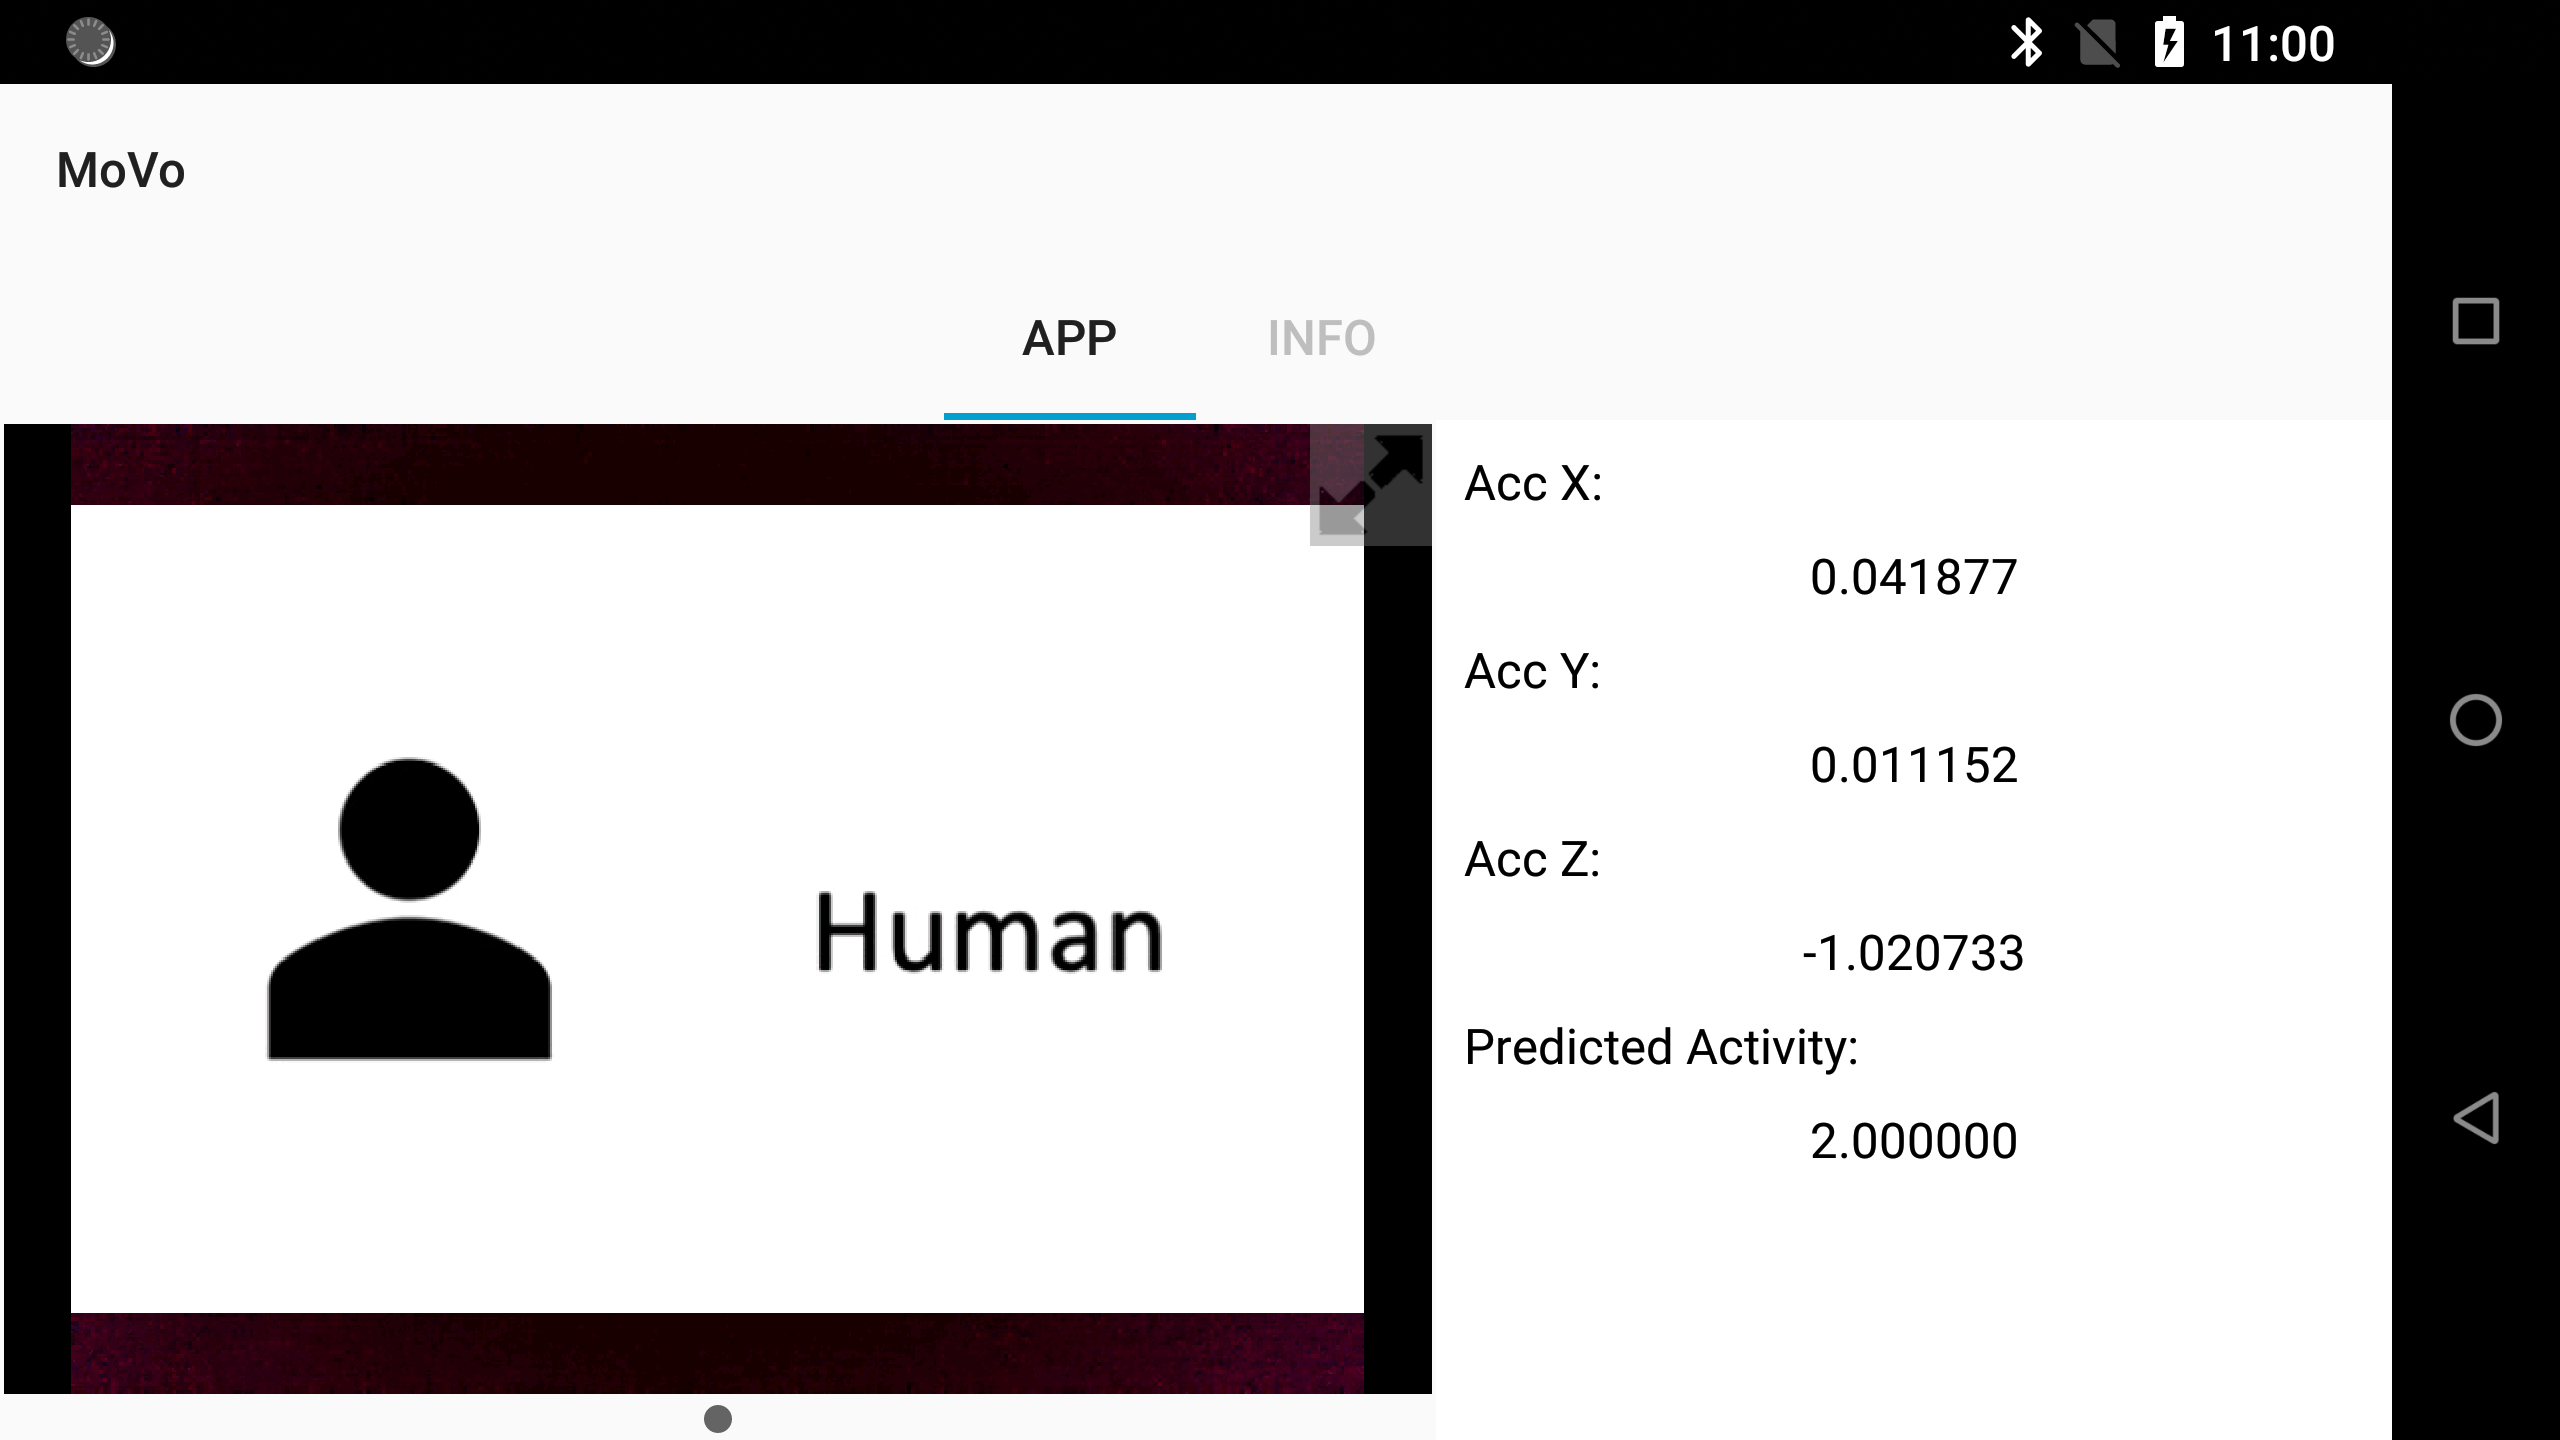
\includegraphics[width=\linewidth]{movohuman}
		\subcaption{Real Person Speaking}
		\vspace{.1in}
		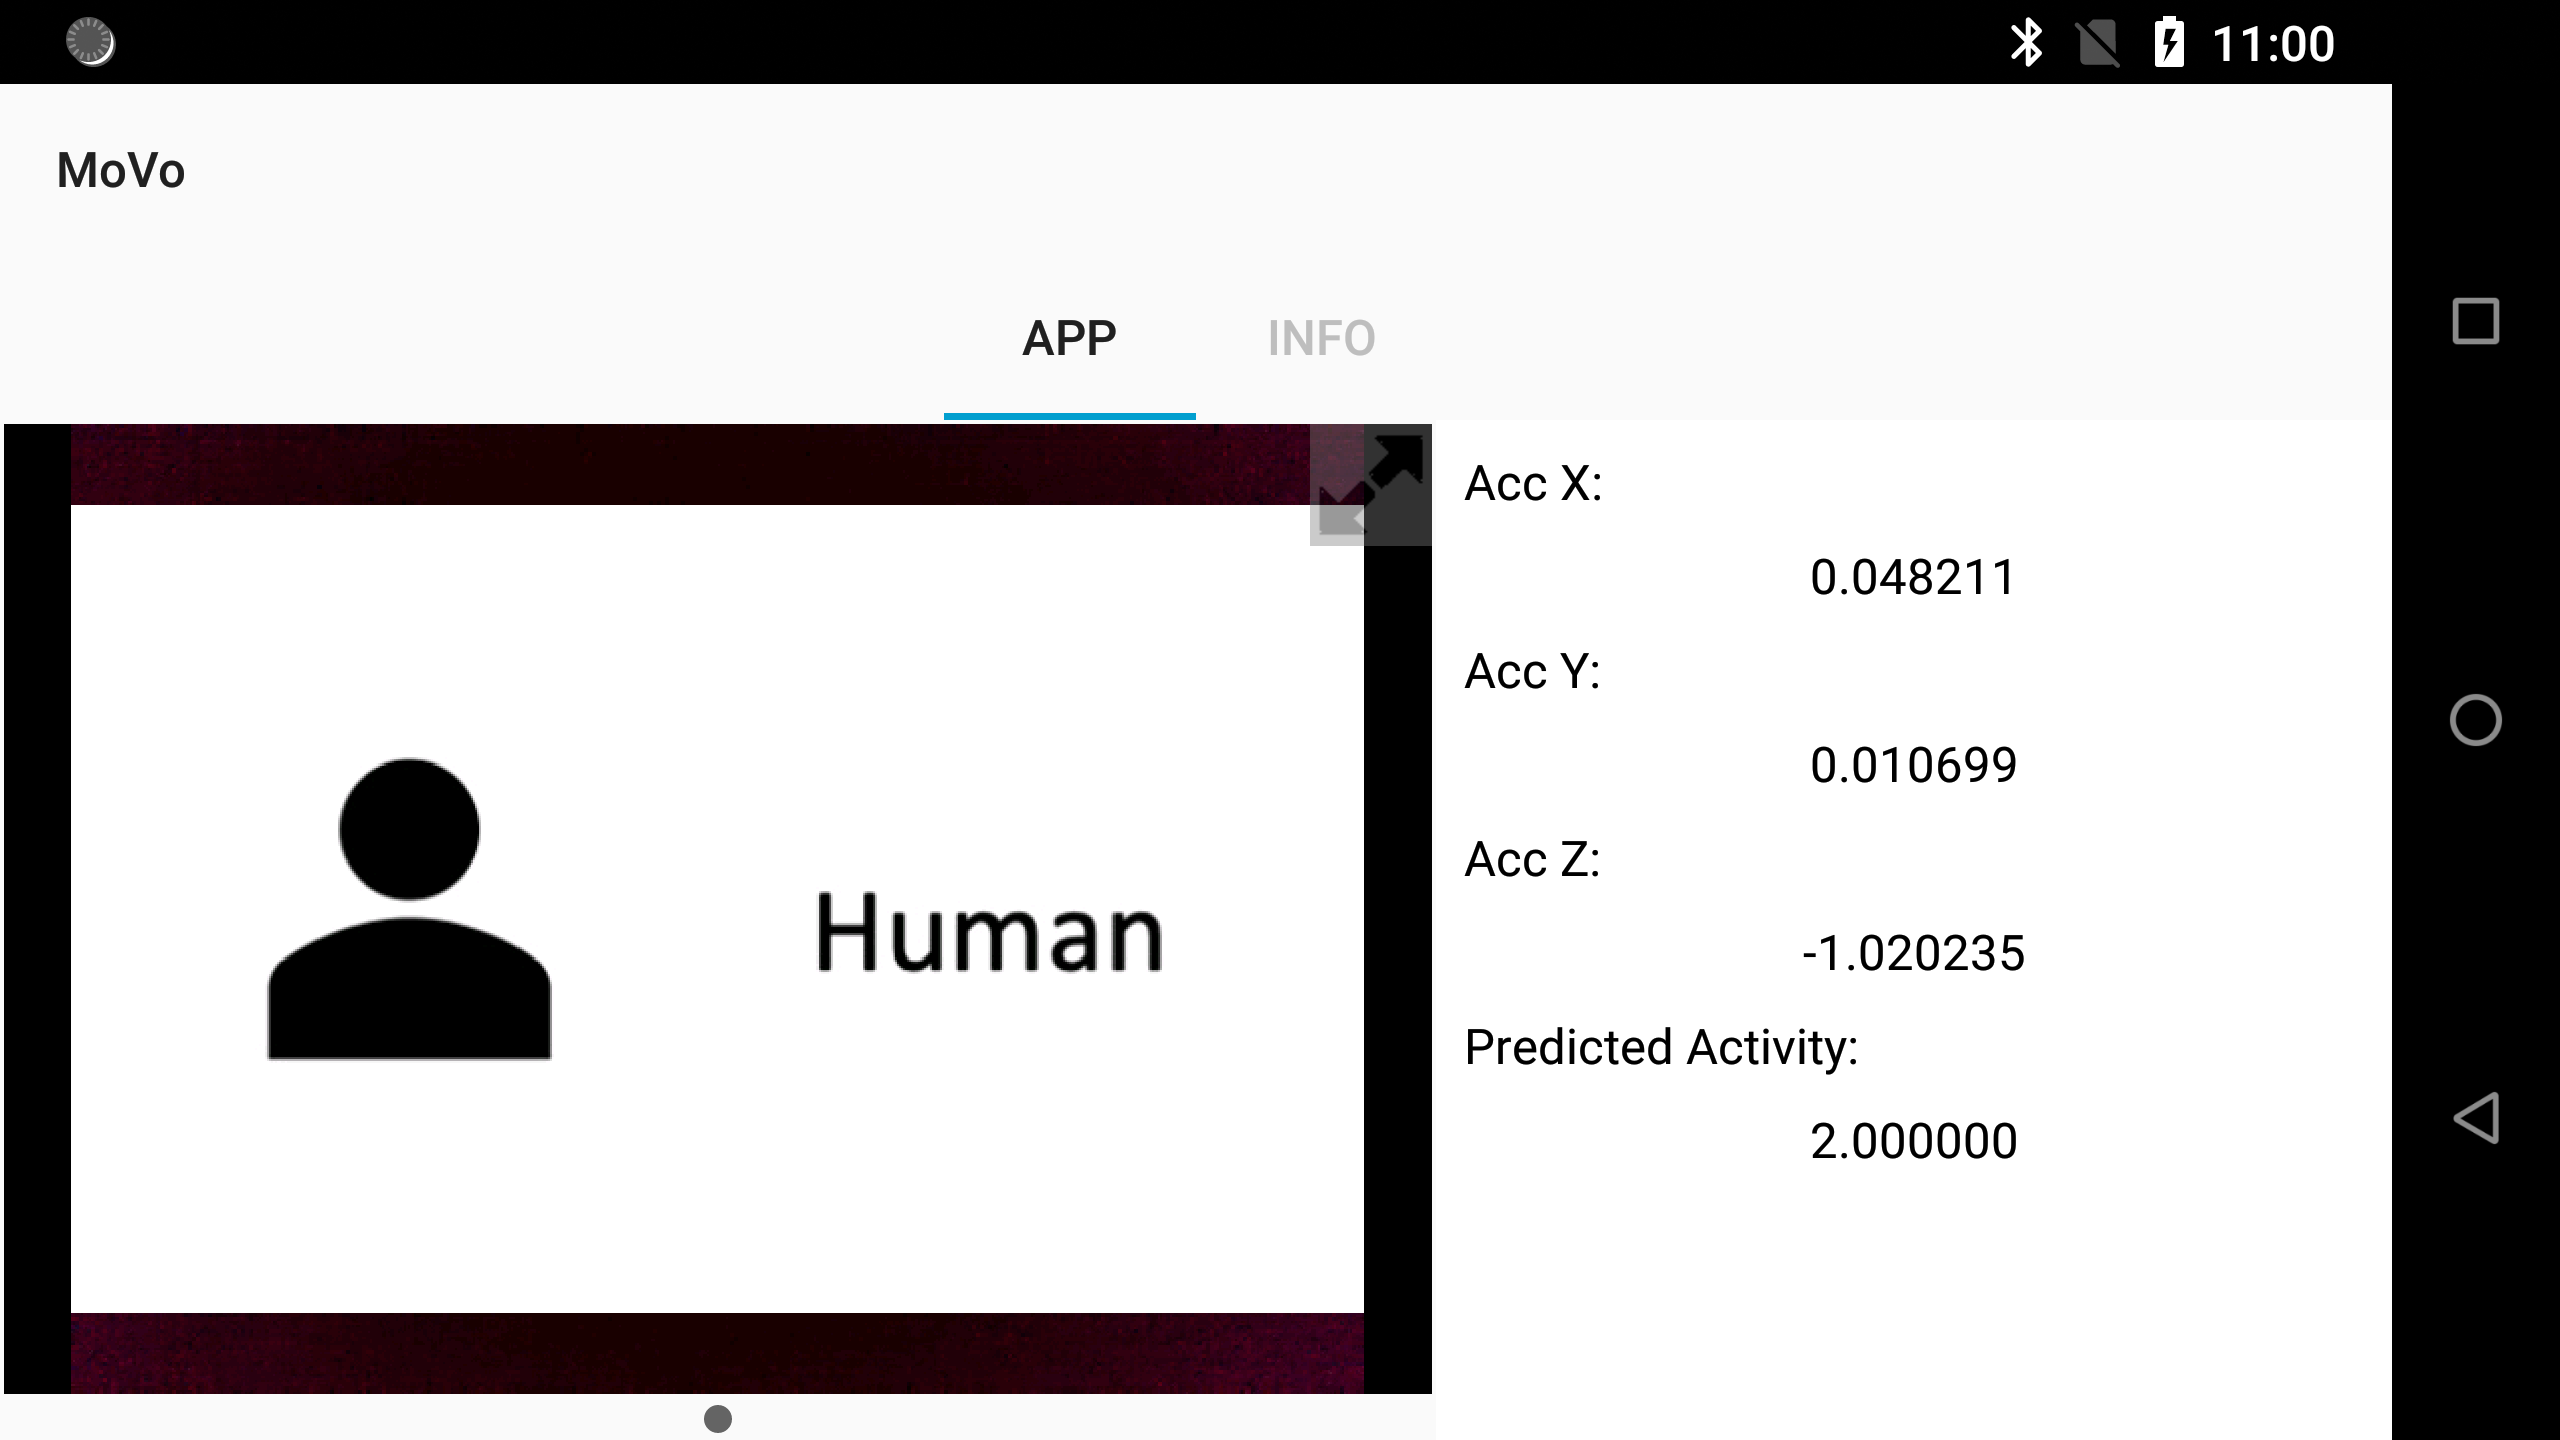
\includegraphics[width=\linewidth]{movodevice}
		\subcaption{Electronic Device Replaying Human Sounds}
		\vspace{.1in}
		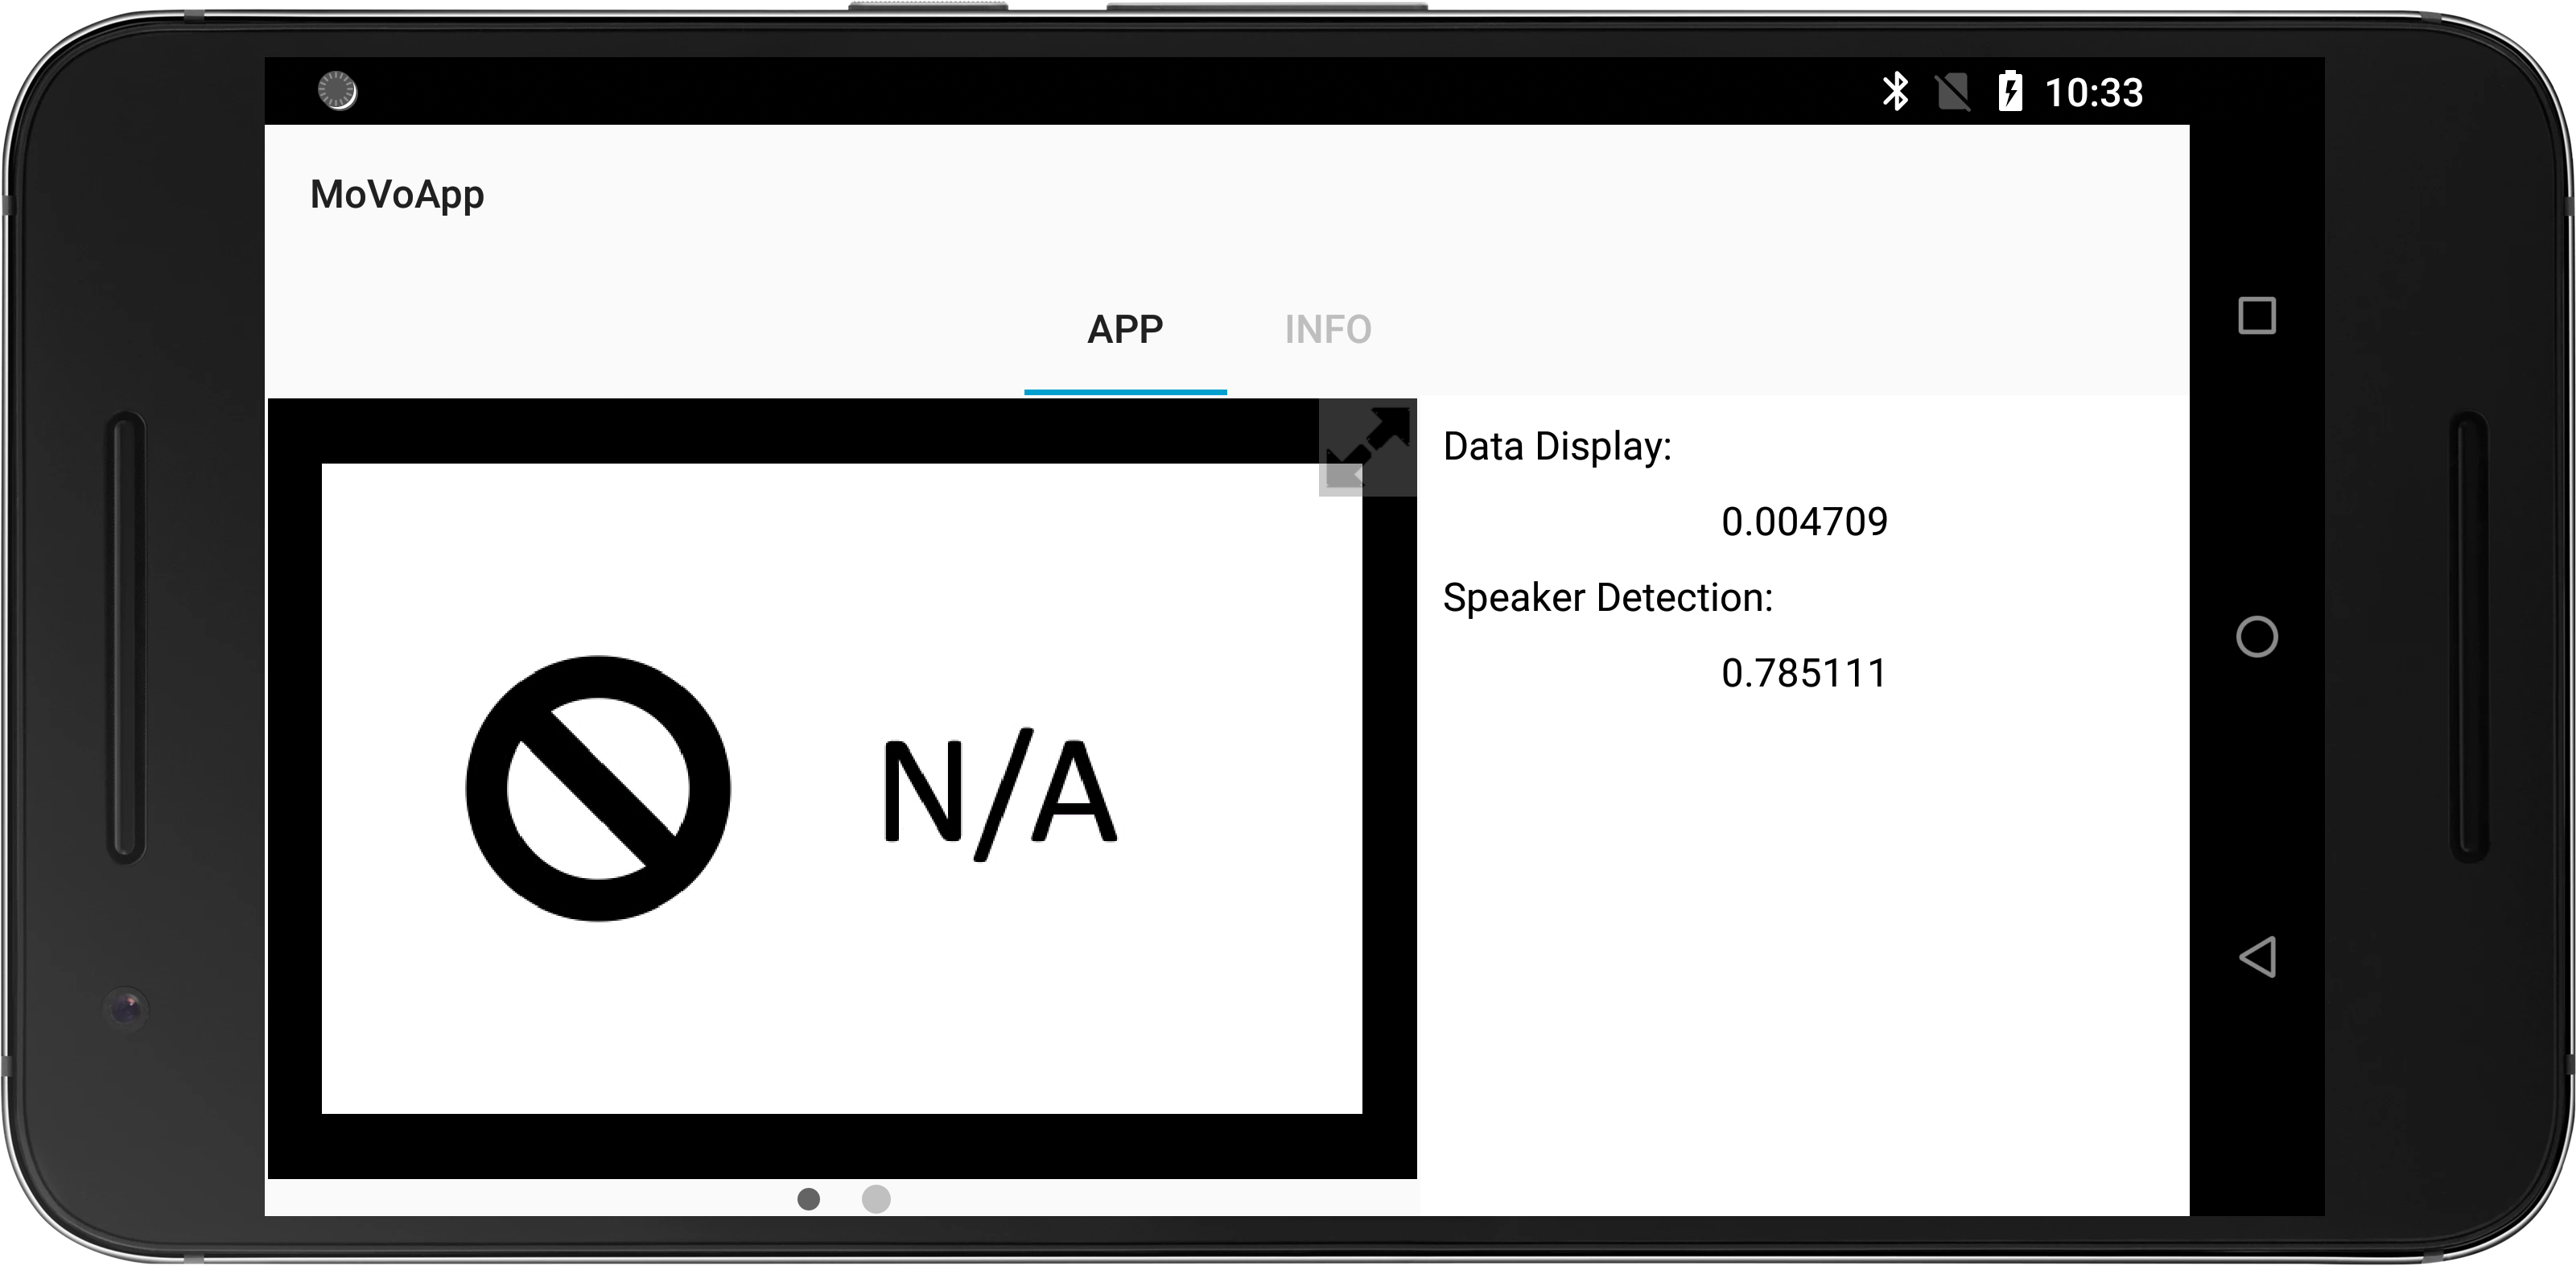
\includegraphics[width=\linewidth]{notapplicable}
		\subcaption{No Human Sounds}
	\end{minipage}
	\caption{Screenshots of the MoVo Data Collection App and MoVo Speaker Detection App}	
	\label{fig:defendapp}
\end{figure}

\textbf{Data Collection}. Our experiment involves 20 participants aged from 20 to 35. Among them, 13 are males and 7 are females; 15 are native English speaker and 5 uses English as a second language. For each user, we ask them to speak the following three hot-words: ``Ok Google'', ``Hi Siri'', and ``Alexa''. For each command, each user repeats it for 5 times. Therefore, we have 300 command samples in total. When we train our LSTM network, we are using the segmented motion data to train 10 different categories (`O', `K', `Goo', `Gle', `Hi', `Si', `Ri', `A', `Le', `Xa'). In this respect, we have 1000 sample sequences, where each sequence is about 100 samples long.


\begin{figure}[!h]
	\centering
	\begin{subfigure}[t]{0.45\textwidth}
		\centering
		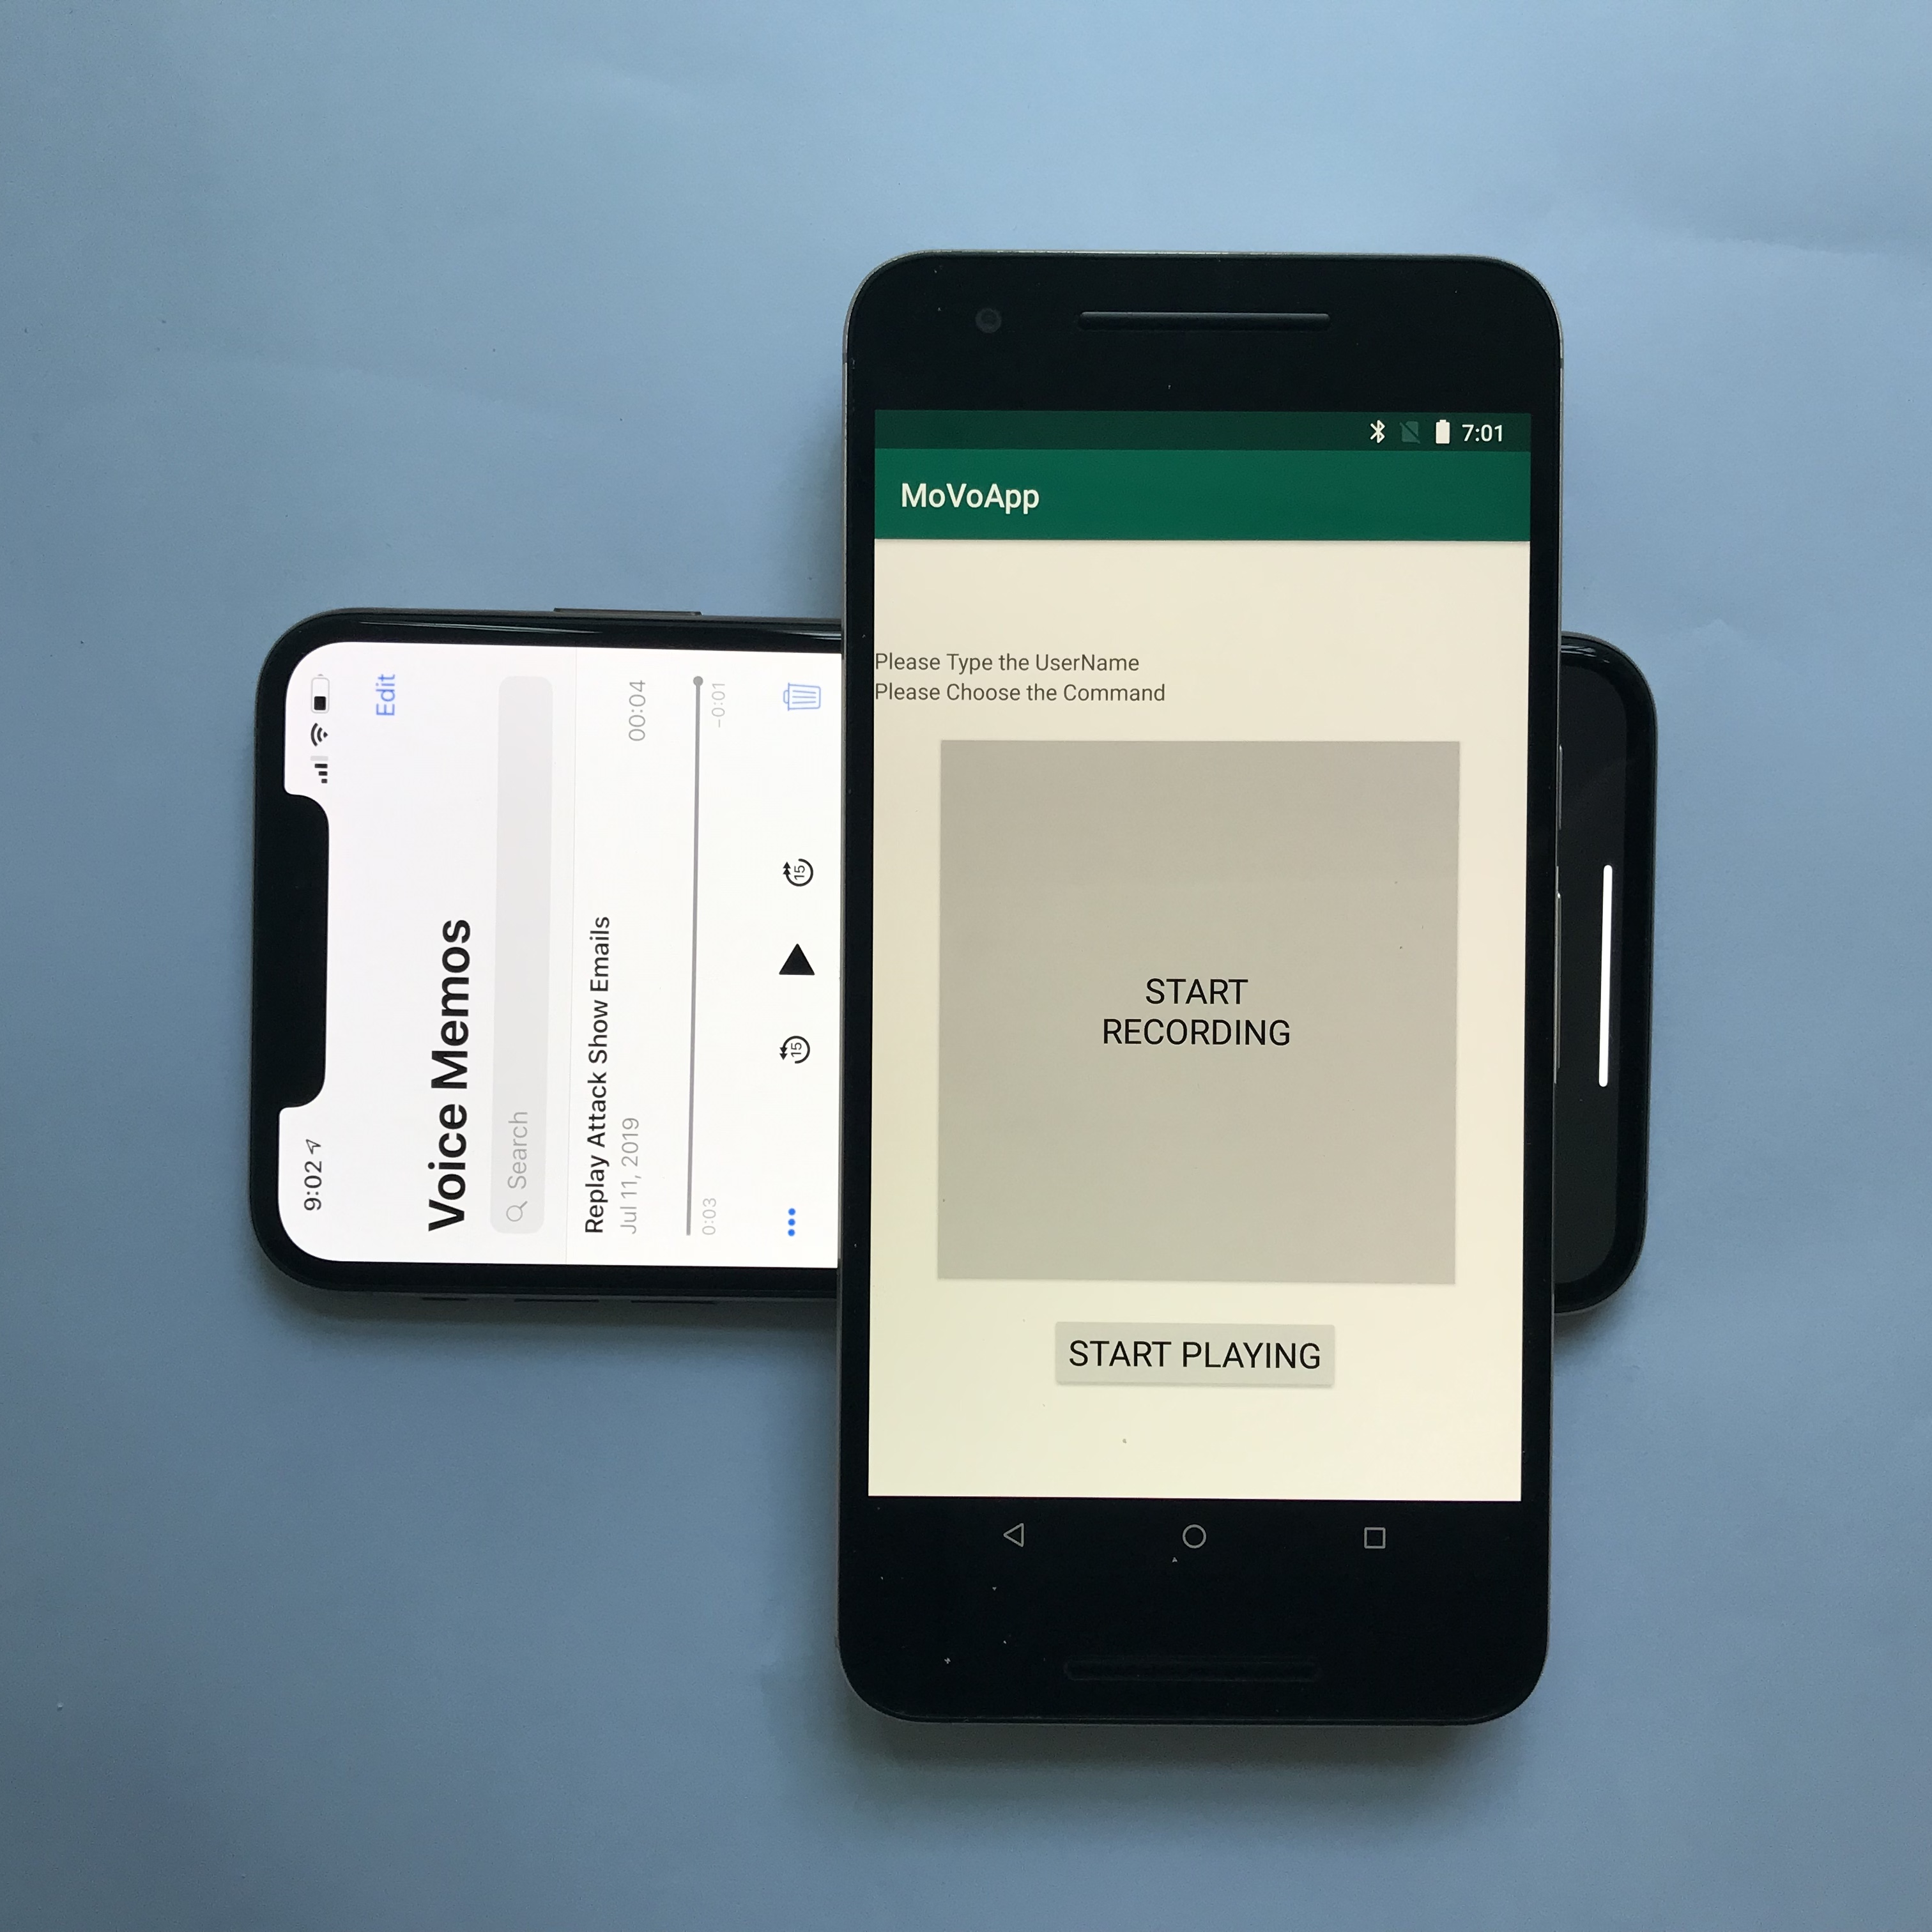
\includegraphics[height=\textwidth]{phone}
		\caption{Smartphone}
	\end{subfigure}%
	~ 
	\begin{subfigure}[t]{0.45\textwidth}
		\centering
		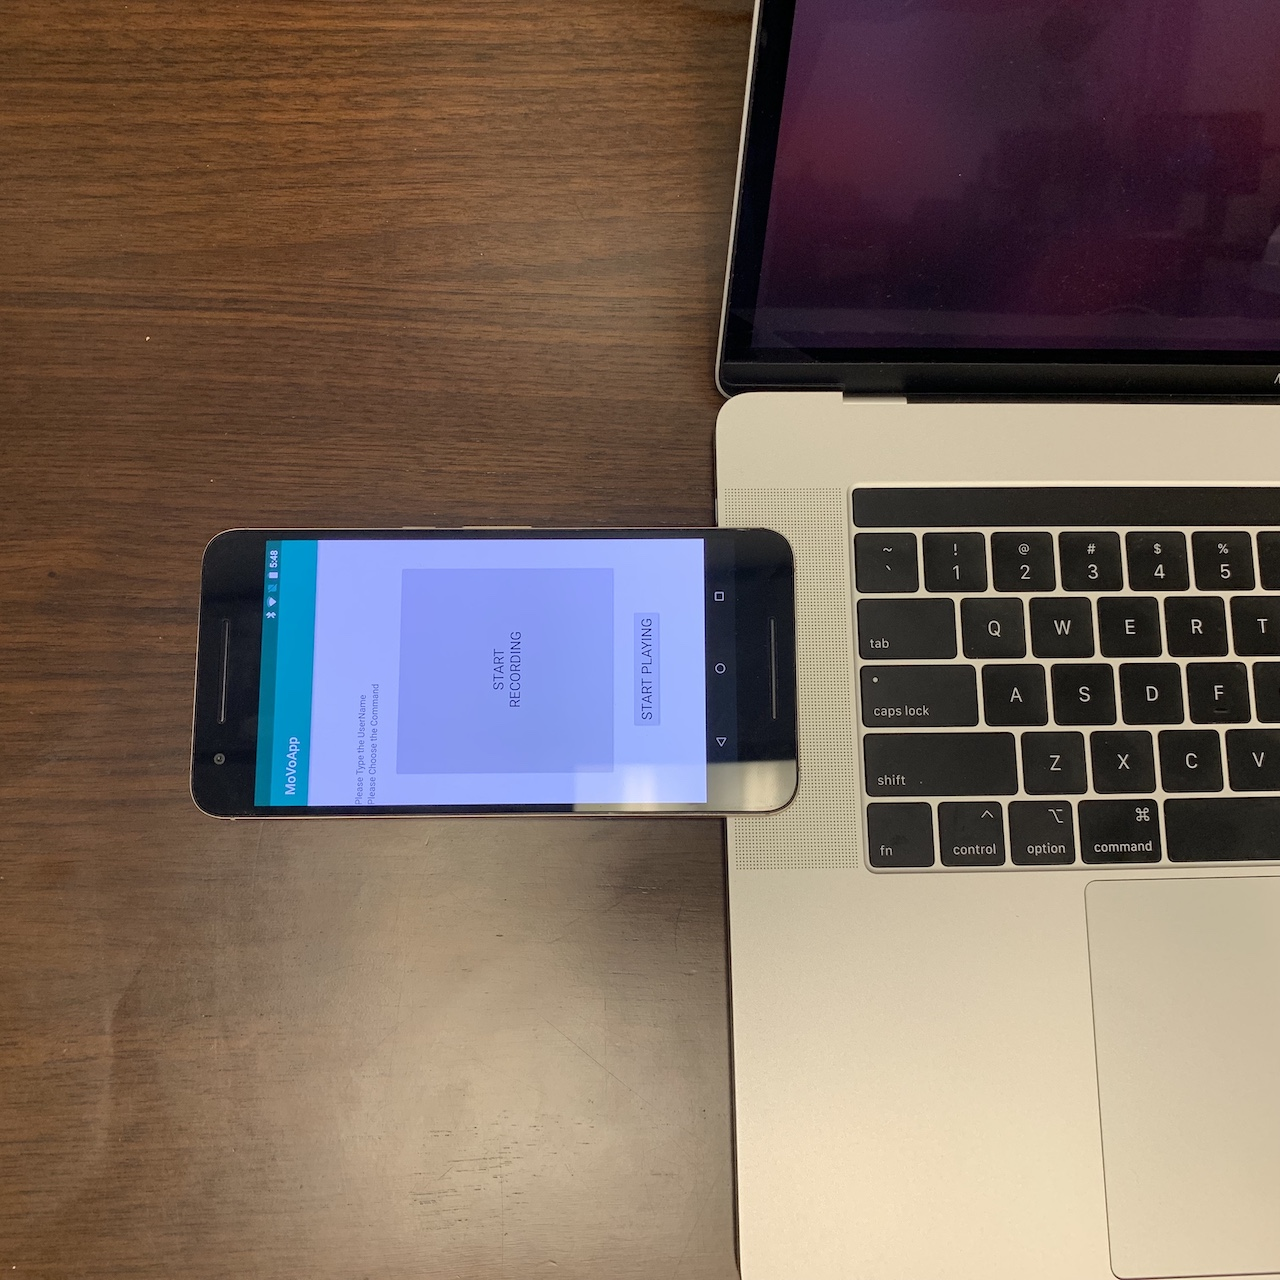
\includegraphics[height=\textwidth]{laptop}
		\caption{Laptop Speaker}
	\end{subfigure}
~ 
\begin{subfigure}[t]{0.45\textwidth}
	\centering
	\includegraphics[height=\textwidth]{desktop}
	\caption{Desktop Speaker}
\end{subfigure}
	~
	\begin{subfigure}[t]{0.45\textwidth}
	\centering
	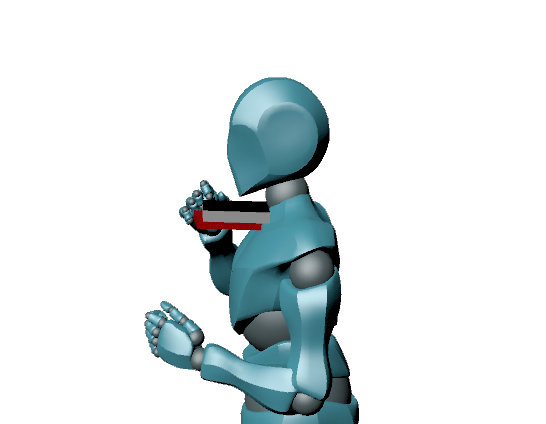
\includegraphics[height=\textwidth]{mimic}
	\caption{Mimicry }
\end{subfigure}
	\caption{Attacker Settings}
	\label{fig:attacks}
\end{figure}





\textbf{Attacks}. As elaborated in Section~\ref{sec:attack}, we evaluate our system against three types of attack scenarios, simple playback attack, mimicry attack and sophisticated mimicry attack, where each scenario contains three kinds of attacks.  Since speech synthesis and voice conversion will generate speech signals similarly if use the same user's speech profile. Therefore, we only test the replay attack.

\begin{figure}[H]
	\centering
	\begin{minipage}{.35\linewidth}
		\includegraphics[width=\linewidth]{movoAttack}
		\vspace{.05in}
	\end{minipage}
	
	\centering
	\begin{tabular}{lr}
		\toprule
		Accuracy: 90.43\% & \hspace{-.55in} Error Rate: 9.57\% \\
		Precision: 90.72\% & \hspace{-.55in} True Positive Rate (Sensitivity/Recall): 90.52\% \\
		$F_1$ Score: 0.904 & \hspace{-.55in} True Negative Rate (Specificity): 95.19\% \\
		False Negative Rate: 9.48\%  & \hspace{-.55in} False Positive Rate: 4.81\% \\
		\bottomrule
	\end{tabular}
	\caption{Success rate of \shortname~on defending against various attacks. }
	\label{fig:defend}
\end{figure}


In simple playback attacks, the recordings of the legitimate user is replayed by either Logitech S120 2.0 Stereo Speakers, the built-in speakers of Apple Macbook Pro, and the built-in speaks of an Apple iPhone XS Max. Each of the 20 participants is considered as a legitimate user separately. For each participant, 5 attacks are conducted by the loudspeaker, 5 attacks are conducted by the laptop speaker, and 5 attacks are conducted by the iPhone speaker. All the three hot-words are tested. In total, there are 450 attacks. The attacking target is always Nexus 6P. The replay sound level is about 80dB, which is in consistent with the decibel level of normal human speech. 
The attacking device and the attacking target  are contacted, so that conductive vibrations are measured. 
In mimicry attacks, two smartphones are placed together and attached to the human throat. In sophisticated mimicry attacks, we consider 2 attackers: one male attacker to mimic the 7 male participants, and the other female attacker to mimic the 3 female participants. The attacker holds the phone tightly to his/her throat while replaying the target user's voice commands as in the simple playback attack cases. The sophisticated mimicry attack is repeated 10 times for each hot-word for each participant. Again, there are 450 such attacks. The final results are shown in Fig.~\ref{fig:defend}, \shortname~can defend replay attack with at least 90.43\% accuracy.

We have also implemented an application on Android to run {\uu} in real-time. As shown in Fig.~\ref{fig:defendapp}, the MoVoApp will decide among the following three cases: 1) a real human is speaking, 2) an electronic device is replaying human speeches, 3) no human sounds are made. Currently, this app only serves as an liveness detection app. We plan to add the user authentication features to this app  in future work. 
\begin{figure}[H]
	\centering
	\begin{minipage}{.35\linewidth}
		\includegraphics[width=\linewidth]{movoCommandbefore}
		\subcaption{Without Majority Voting}\label{fig:commadmata}
		\vspace{.05in}
	\end{minipage}
	\begin{minipage}{.35\linewidth}
		\includegraphics[width=\linewidth]{movoCommandafter}
		\subcaption{With Majority Voting}\label{fig:commadmatb}
		\vspace{.05in}
	\end{minipage}
	
	\centering
	\begin{tabular}{lr}
		\toprule
		Accuracy: 93.67\% & \hspace{-.55in} Error Rate: 6.33\% \\
		Precision: 93.67\% & \hspace{-.55in} True Positive Rate (Sensitivity/Recall): 93.71\% \\
		$F_1$ Score: 0.937 & \hspace{-.55in} True Negative Rate (Specificity): 96.84\% \\
		False Negative Rate: 6.29\%  & \hspace{-.55in} False Positive Rate: 3.16\% \\
		\bottomrule
	\end{tabular}
	\caption{Confusion Matrix of Matching Motion Data to Different Hot-Words. }
	\label{fig:commadmat}
\end{figure}


\textbf{Results}.
%
Besides defending against various attacks, \shortname~should accept legitimate users as in normal voice authentication systems. In other words, \shortname~should correctly classify a legitimate user's motion data to the hot-words he says. As shown in Fig.~\ref{fig:commadmat}, the overall accuracy of correct classification is 93.67\%.  
Note that we have two confusion matrices. Figure~\ref{fig:commadmata} is the original results provided by the machine learning network, while Figure~\ref{fig:commadmatb} is the result with majority voting procedure. There is a significant accuracy improvement with the presence of majority voting. Therefore, we only show the statistic evaluations of Figure~\ref{fig:commadmatb}. 


\begin{table}[t]
	\caption{Statistical Analysis of the User Classification Result}
	\label{tab:userTable}
	\centering
	\begin{tabular}{lr}
		\toprule
		Accuracy: 92.98\% & \hspace{-.55in} Error Rate: 7.02\% \\
		Precision: 93.33\% & \hspace{-.55in} True Positive Rate (Sensitivity/Recall): 94.58\% \\
		$F_1$ Score: 0.924 & \hspace{-.55in} True Negative Rate (Specificity): 99.64\% \\
		False Negative Rate: 5.42\%  & \hspace{-.55in} False Positive Rate: 0.36\% \\
		\bottomrule
	\end{tabular}
\end{table}



\begin{figure}[h]
	\centering
	\includegraphics[width=.5\linewidth]{movoTime}
	\caption{Robustness of {\shortname} over time.}
	\label{fig:time}
\end{figure}



The results for user authentication are shown in Fig.~\ref{fig:usermat} and Table.~\ref{tab:userTable}. Without majority voting, the accuracy of user authentication is only 54.48\%. With majority voting, the accuracy increases to 92.98\%. Note that this accuracy cannot beat existing speaker recognition systems based on audio files. Therefore, for better security, this result can serve as an extra channel of information. 

We also test the robustness of {\shortname} in Fig.~\ref{fig:time}. We test both the one-time trained model and the learning model which will use the accepted data as trained data for future authentication. Over 8 weeks, the learning model has more stable performance.






%We also evaluate the impact of feature dimensions on the classification accuracy. When we train the sequence-to-sequence LSTM network, we use all six dimensions of the motion data. In fact, different dimensions impact the classification result differently. As shown in Fig.~\ref{fig:axis}, accelerometer data are more useful in the classification than the gyroscope data. The more dimensions we use, the higher accuracy we can achieve. Among all single dimensions, the z direction of accelerometer is the best, which is the direction perpendicular to human throat surface. This is because the vibration on this direction is larger and easier to be caught by the accelerometer.
%
%\begin{figure}[h]
%	\centering
%%	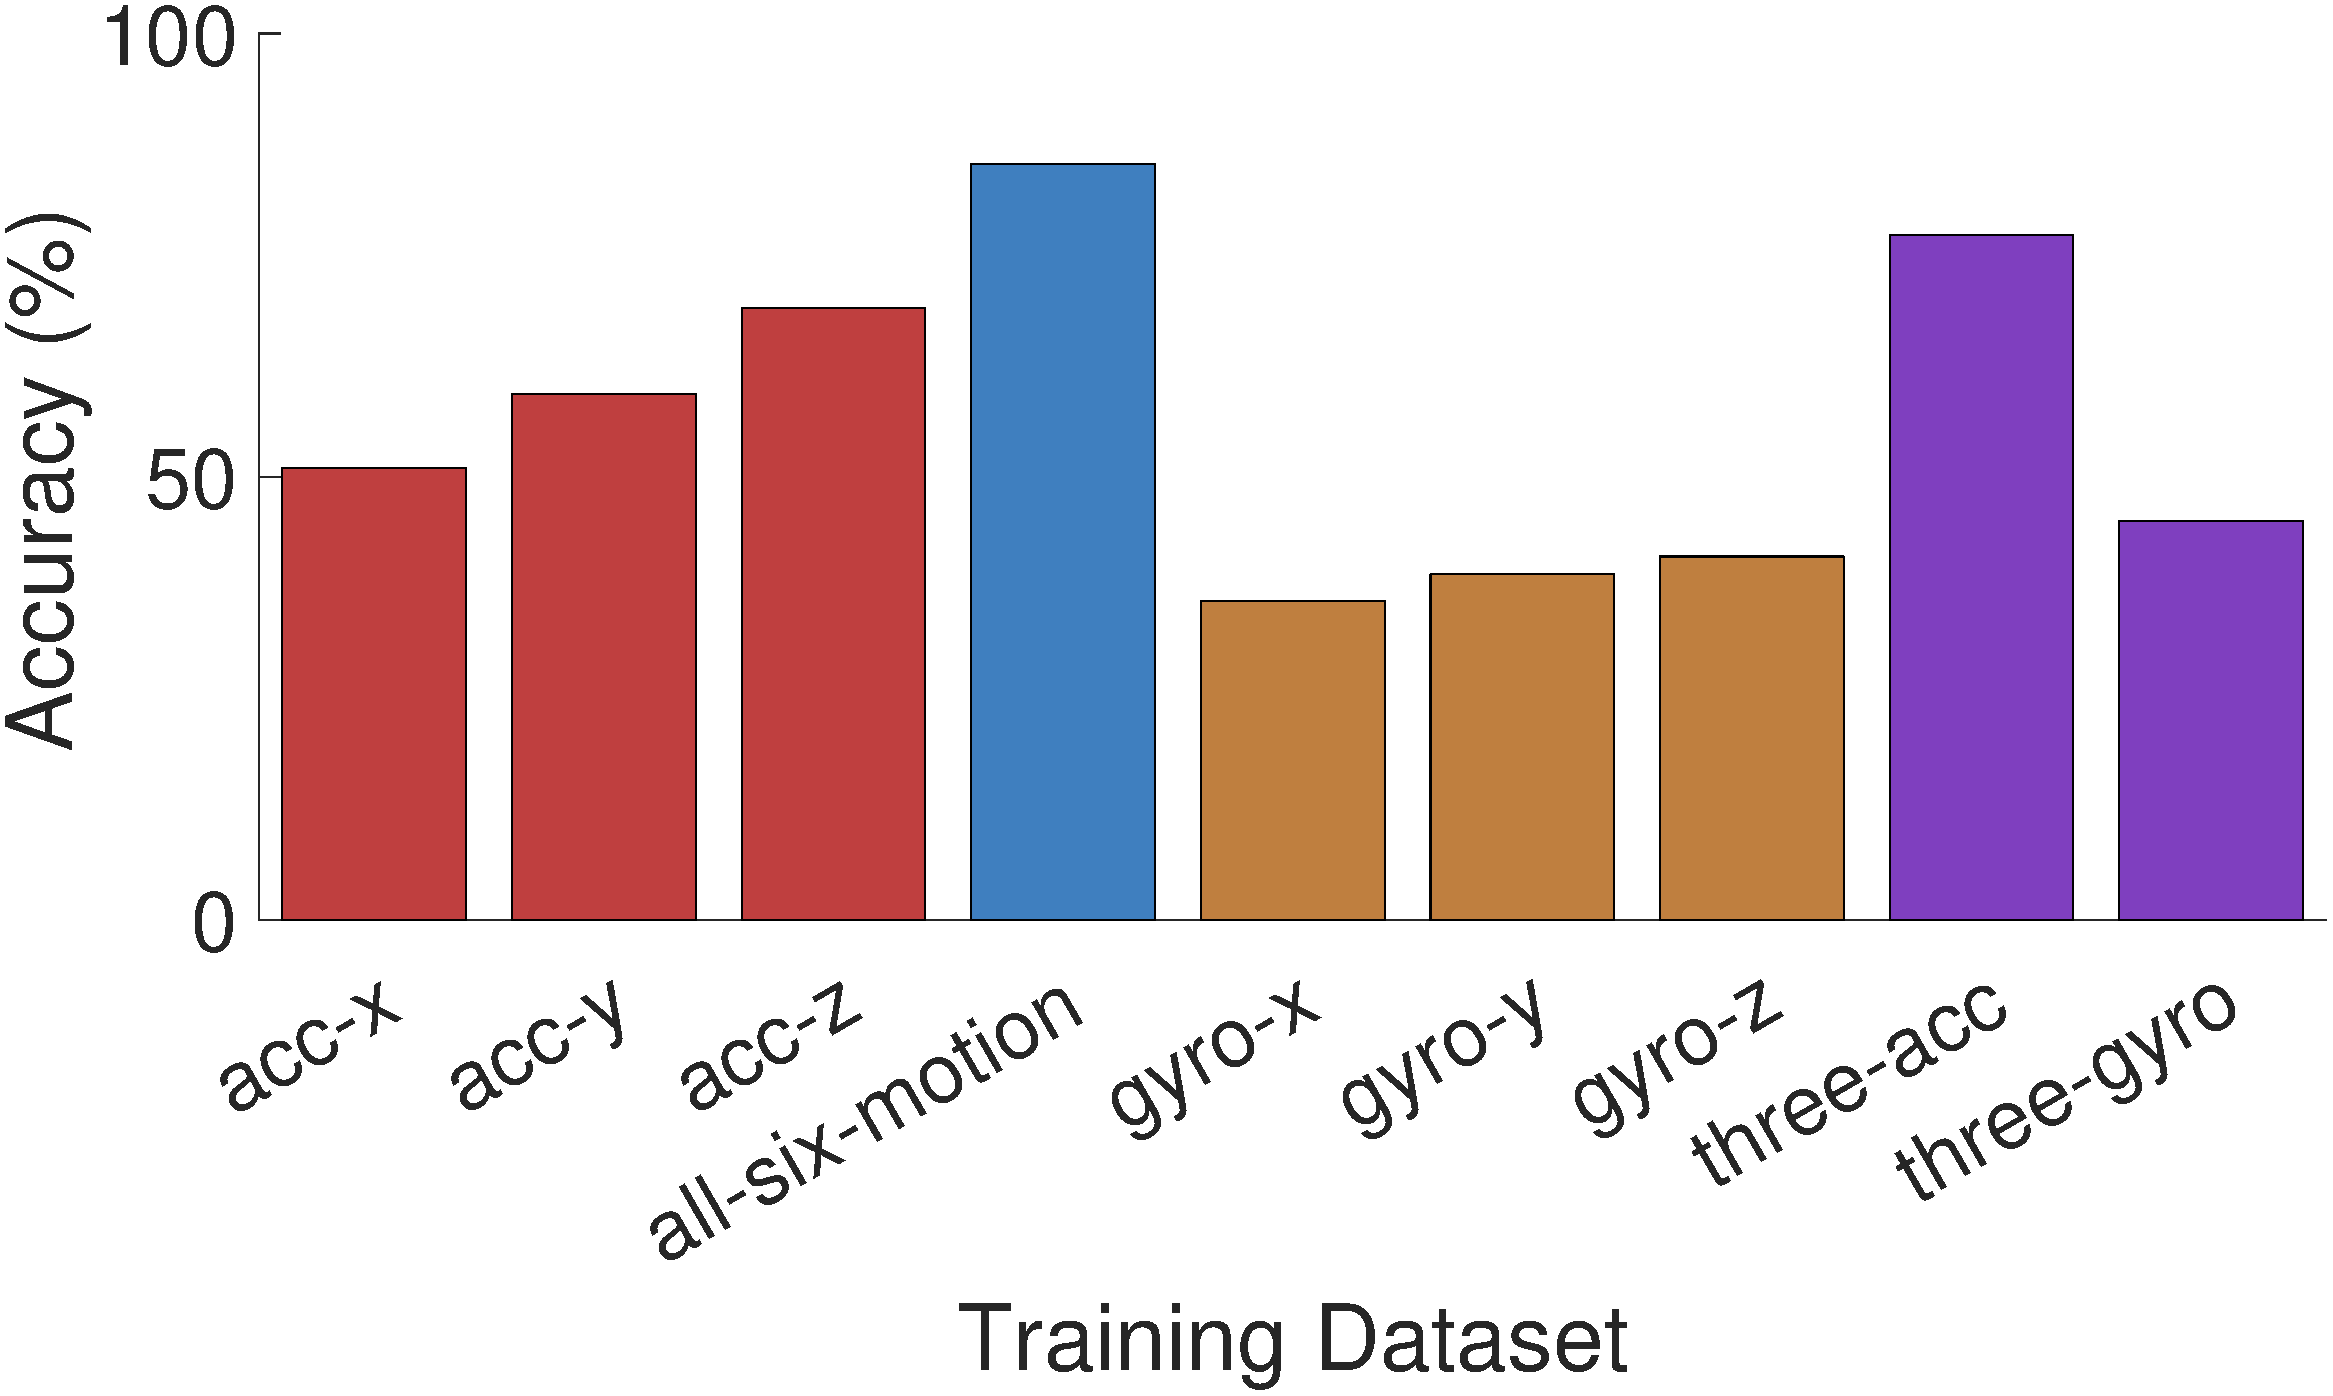
\includegraphics[width=.6\linewidth]{axis}
%	\caption{Classification accuracy using different feature dimensions in the sequence input layer of our LSTM network.}
%	\label{fig:axis}
%\end{figure}







%\textbf{Discussion}. 
%Our \shortname~have some limitations. For example,  the number of evaluation participants and the size of hot-words dataset are relatively small. A larger dataset can be very useful to help evaluate the system though the technique contribution is limited. Another limitation is the overall classification accuracy. This shortcoming can be easily overcome by building a user-dependent classification model instead of the current user-independent one.  We have tested on the same dataset and found that the classification accuracy increases from 85.3\% to 93.7\% as shown in Fig.~\ref{fig:depenmat}. 

%\begin{figure}[H]
%	\centering
%	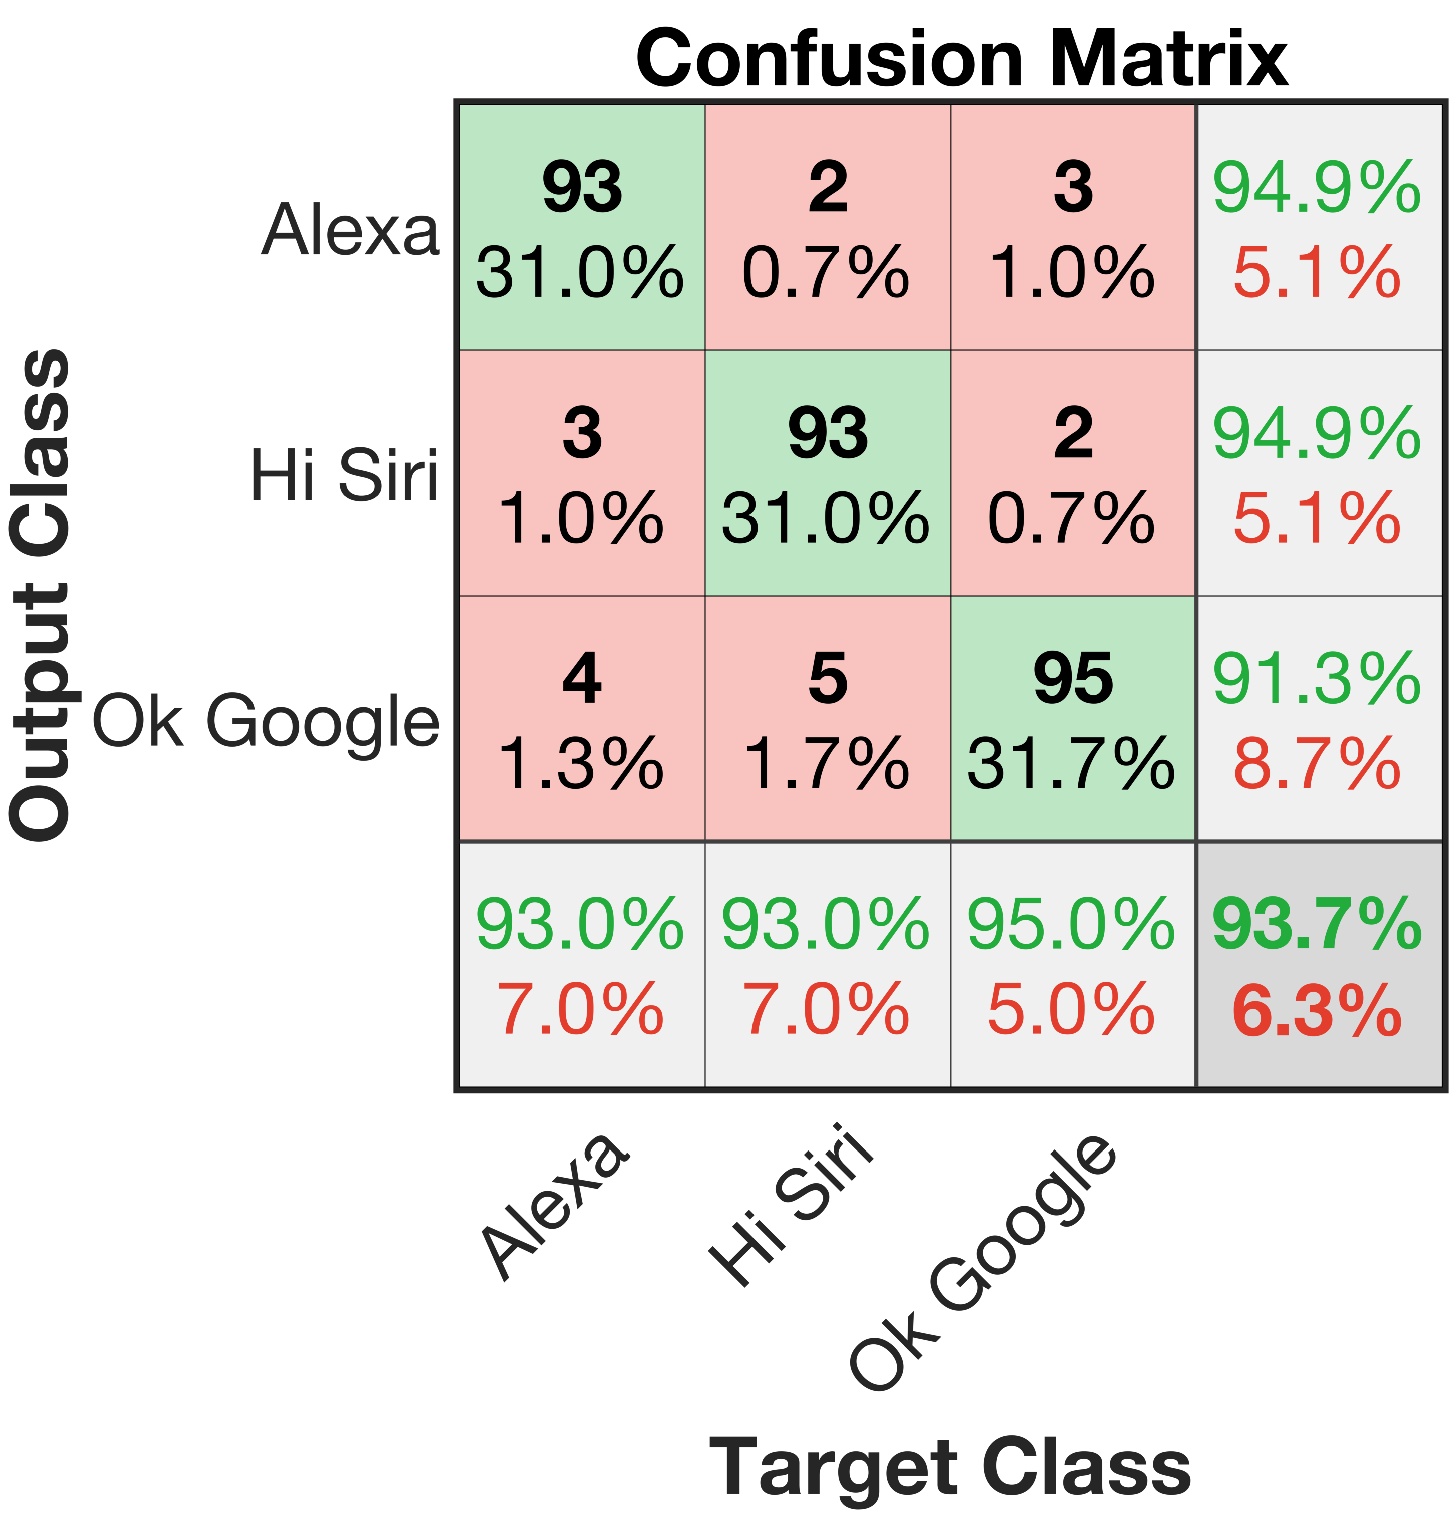
\includegraphics[width=.4\linewidth]{depenmat}
%	\caption{Confusion matrix of matching motion data to different hot-words when training the user-dependent LSTM model.}
%	\label{fig:depenmat}
%\end{figure}
%TODO more evaluation
%\begin{itemize}
%\item
%Evaluate different gender
%\item
%Evaluate user-dependent
%\item
%Evaluate Walking-Sitting-Running
%\item
%Evaluate syllable separation vs. process as a whole
%\item
%Evaluate high pass filter
%\item
%Evaluate majority voting
%\item
%compare with other algorithms (Spinx, SVM,...)
%\item
%Evaluate against different smartphones
%\item
%More person
%\end{itemize}


%Currently, we have implemented 4 traditional features (min, max, skewness, std. deviation)  and test the accuracy on 3 commands (‘Hi Siri’ and ‘Ok Google’). In total, we have 180 samples and each has a feature vector of length 32. By using the MATLAB classification app, we could achieve the maximum accuracy of 89%, which is achieved by the Quadratic Support Vector Machines.

%
